%%%%%%%%%%%%%%%%%%%%%%%%%%%%%%%%%%%%%%%%%%%%%%%%%%%%%%%%%%%%%%%%%%%%%%%%%
% This file is part of the LaTeX sources of the OMDoc 1.6 project descriptions
% Copyright (c) 2006 Normen Mueller
% This work is licensed by the Creative Commons Share-Alike license
% see http://creativecommons.org/licenses/by-sa/2.5/ for details
% The source original is at https://github.com/KWARC/OMDoc/doc/projects/verifun
%%%%%%%%%%%%%%%%%%%%%%%%%%%%%%%%%%%%%%%%%%%%%%%%%%%%%%%%%%%%%%%%%%%%%%%%%

\begin{omgroup}[id=verifun,short=VeriFun,creators={nmueller}]
  {{\omdoc} as a Data Format for {\verifun}}

\ednote{project page:\url{http://www.verifun.de/}}

{\verifun} (\underline{Ver}ification of \underline{Fun}ctional programs) is a
semi-automated system for the verification of programs written in a simple functional
programming language {\fp}. The system has been developed since 1998 at the university of
Darmstadt for use in education and research. The main design goals are a clearly
structured, didactically suited system interface (\myfigref{verifun}), an easily portable
implementation ({\java}) and an easily
\begin{wrapfigure}{r}{8cm}\vspace*{-.3cm}
  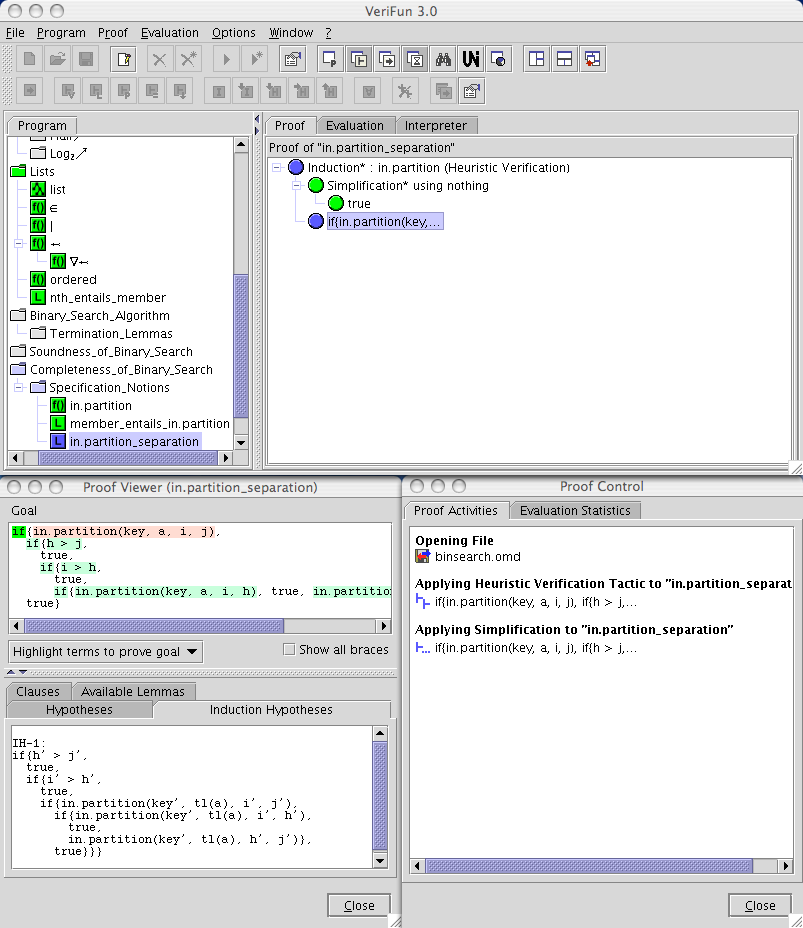
\includegraphics[width=8cm]{\projectsPath{verifun/verifun}}
  \label{fig:verifun}\caption{A {\verifun} session}\vspace*{-.3cm}
\end{wrapfigure}
but also powerful proof calculus~\cite{WS:VFTut}. The system's object language consists of
a simple definition principle for free data structures, called {\emph{sorts}} (see
{\extref{spec}{adt}}), a recursive definition principle for {\emph{functions}}, and
finally a definition principle for statements, called {\emph{lemmas}}, about the data
structures and the functions. To prove a statement {\verifun} supports the user with a
couple of inference rules aggregated in {\emph{tactics}}. A collection of {\emph{sorts}},
{\emph{functions}}, {\emph{lemmas}}, and {\emph{proofs}} is called a {\verifun}
{\emph{program}}. Common file commands, which are based on the {\java} binary
serialization mechanism, are provided to save and reload intermediate work.

The {\omdoc} interface for {\verifun} described here (see~\cite{NRM:DA05} for details) was
introduced to alleviate the following drawbacks of the former I/O mechanism based on
{\java} binary serialization:
\begin{itemize}
\item Files are only machine-readable. Thus, e.g. if the files became corrupted by any
  circumstance, there is no change of a manual repair.
\item Files are strongly bound to the version of the system. Thus any internal system
  modifications make the files unreadable.
\item Files are not interchangeable with other theorem provers or other mathematical
  software systems. Thus the information inside the files are only accessible by
  {\verifun}.
\end{itemize}

{\verifun}'s interface to {\omdoc} can be divided into two parts: Encoding and decoding of
{\verifun} programs to and from {\omdoc} respectively.

\begin{omgroup}{Encoding}

In a typical session with the system, a user defines a {\emph{program}} by stipulating the
{\emph{sorts}} and the {\emph{functions}} of the program, defines {\emph{lemmas}} about
the sorts and the functions of the program, and finally verifies these lemmas and the
termination of the functions.

In general a {\emph{program}} is mapped to two {\omdoc} files: The first one consists of
the user-defined elements\footnote{Actually there are also automatically system-generated
  elements included, but we may neglect those at this point.} and in the second one
{\mbox{{\verifun}'s}} logic comprising the predefined symbols, the type system and the
proof tactics is defined. At each case one {\verifun}-generated-{\omdoc} file is composed
of one {\element{theory}} element. The name of a user-defined theory can be set by the
user, whereas the name of the theory {\mbox{\verifun}} is based on is fixed to
{\sc{vafp}}.

{\emph{Functions}} are declared by {\element{symbol}} elements that also introduces the
type of the function (\extref{spec}{type-axioms}).  The body of a function is encoded as
an {\openmath} object inside a {\element{definition}} element. The corresponding
{\element{symbol}} element is referenced by the {\element{definition}} element in the
{\attribute{for}{definition}} and relating termination assertions in the
{\attribute{existence}{definition}} attribute.

Note that instead of using {\attribute{name}{symbol}} attributes, which only allow {\xml}
simple names, we generate a unique {\sc{ID}}. The actual {\verifun} names are represented
in {\element{presentation}} elements or rather their {\element{use}} elements
(\mylstref{omdoc:pres}). By using this technique we can use any character
string\footnote{{\verifun} has full {\unicode}~\cite{Unicode:tuc03} support} for element
names. To cover the whole set of {\verifun} fixities
({\attval{prefix}{fixity}{presentation}} (the default),
{\attval{infix}{fixity}{presentation}}, {\attval{postfix}{fixity}{presentation}},
{\attval{infixl}{fixity}{presentation}}, {\attval{infixr}{fixity}{presentation}}, and
{\attval{outfix}{fixity}{presentation}}) we had to extend the {\omdoc} format by
{\attval{infixl}{fixity}{presentation}} and
{\attval{infixr}{fixity}{presentation}}. However, it was not necessary to also add the
{\attval{outfix}{fixity}{presentation}} value, but encoding of
{\attval{outfix}{fixity}{presentation}} functions is treated slightly different: The name
of the function is encoded in the {\attribute{lbrack}{presentation}} and
{\attribute{rbrack}{presentation}} attribute respectively of the relating
{\element{presentation}} element and the {\element{use}} element is left empty\footnote{As
  a consequence the previous mentioned special encoding feature does not hold for outfix
  functions}.

{\emph{Lemmata}} are mapped to {\element{assertion}} elements, the value
``{\attval{lemma}{type}{assertion}}'' being assigned to the {\attribute{type}{assertion}}
attribute. The formula of a lemma, analogous to function bodies, is encoded as an
{\openmath} object inside an {\element{assertion}} element.

Particularly convenient is the direct mapping of {\verifun} proofs to the {\omdoc}
presentation of proofs. Verifications of lemmas and termination analysis of functions are
represented in {\element{proof}} elements. The assertion to be proven is referenced in the
{\attribute{for}{proof}} attribute. {\sc{vafp}}-tactics used inside a proof to achieve the
various proof steps (encoded in {\element{derive} elements}) are denoted by
{\element{method}} elements. Parameters heuristically computed by the system or manually
annotated by the user are encoded as {\openmath} objects and appended to each proof
step. Furthermore each proof step in {\verifun} is annotated with a sequence of the form
$h_1, \dots h_n, \forall \dots ih_1, \dots, \forall \dots ih_l \vdash goal$ whereas the
expressions $h_i$ are the hypotheses, the expressions $\forall \dots ih_k$ are the
induction hypotheses, and the expression $goal$ is the goal-term of the sequence. Such a
sequent is represented by {\element{assumption}} and {\element{conclusion}} child-elements
respectively of the relating {\element{derive}} element.
\begin{lstlisting}[escapechar=\%,mathescape,label=lst:vf:adt,caption={A polymorphic {\verifun} sort}]
structure list[@value] <=
  $\emptyset$,
  [infixr,100] ::(hd : @value, tl : list[@value])
\end{lstlisting}

{\emph{Sorts}} are wrapped inside {\element{adt}} elements. At this point this integration
process provoked two further adaptations of the {\omdoc} standard. On the one hand, in
contrast to {\omdoc}, sorts in {\verifun} could be polymorphic (\mylstref{vf:adt}). This
led to the additional, optional {\attribute{parameters}{adt}} attribute of an
{\element{adt}} element (\mylstref{omdoc:adt}). Within this new attribute one can declare
by a comma separated list the names of type variables of the abstract data type.
\begin{lstlisting}[label=lst:omdoc:adt,caption={A polymorphic {\omdoc} ADT}]
<adt xml:id="vf7b9f3e59-e78e-4221-8064-7fa0c5689f5d.adt" parameters="value">
  <sortdef name="vf7b9f3e59-e78e-4221-8064-7fa0c5689f5d" type="free">
    <constructor name="vf8a6673ac-c1d9-4698-b6ee-90213539a984"/>
    <constructor name="vf38164505-4983-417f-8bdc-6a42b046e933">
      <argument>
        <type system="simpletypes">
          <OMOBJ xmlns="http://www.openmath.org/OpenMath">
            <OMV name="value"/>
          </OMOBJ>
        </type>
        <selector name="vf9fc4c672-207f-45c0-ae61-1f675fde7aed" total="yes"/>
      </argument>
      <argument>
        <type system="simpletypes">
          <OMOBJ xmlns="http://www.openmath.org/OpenMath">
            <OMA>
              <OMS cd="VeriFun" name="vf7b9f3e59-e78e-4221-8064-7fa0c5689f5d"/>
              <OMV name="value"/>
            </OMA>
          </OMOBJ>
        </type>
        <selector name="vf55767f3a-b019-4308-88f9-d68ee0db595e" total="yes"/>
      </argument>
    </constructor>
  </sortdef>
</adt>
\end{lstlisting}
On the other hand, the child elements of a {\element{constructor}} element had to be
expanded by an additional {\element{type}} element to specify the type of the formal
parameter of the parent {\element{constructor}} element. {\mylstref{omdoc:pres}}
illustrates the corresponding {\element{presentation}} elements of the ADT in
{\mylstref{omdoc:adt}}.
\begin{lstlisting}[escapechar=\%,mathescape,label=lst:omdoc:pres,caption={Representation of {\verifun} names to {\omdoc}}]
<presentation for="#vf7b9f3e59-e78e-4221-8064-7fa0c5689f5d" role="applied">
  <use format="VeriFun">list</use>
</presentation>
<presentation for="#vf8a6673ac-c1d9-4698-b6ee-90213539a984" role="applied"
               bracket-style="math" precedence="1" fixity="prefix" lbrack="(" rbrack=")">
  <use format="VeriFun">$\emptyset$</use>
</presentation>
<presentation for="#vf38164505-4983-417f-8bdc-6a42b046e933" role="applied" 
               bracket-style="math" precedence="100" fixity="infixr" lbrack="(" rbrack=")">
  <use format="VeriFun">::</use>
</presentation>
<presentation for="#vf9fc4c672-207f-45c0-ae61-1f675fde7aed" role="applied"
               bracket-style="math" precedence="1" fixity="prefix" lbrack="(" rbrack=")">
  <use format="VeriFun">hd</use>
</presentation>
<presentation for="#vf55767f3a-b019-4308-88f9-d68ee0db595e" role="applied"
               bracket-style="math" precedence="1" fixity="prefix" lbrack="(" rbrack=")">
  <use format="VeriFun">tl</use>
</presentation>
\end{lstlisting}  
\end{omgroup}

\begin{omgroup}{Decoding}

The decoding of a {\verifun} program represented in {\omdoc} is reverse to the encoding
mechanism. First we create an empty program and then start the sequential decoding of each
{\element{adt}}, {\element{symbol}} and its relating {\element{definition}}, and
{\element{assertion}} element back into the {\fp} syntax. After a successful
reconstruction of an element it is appended to the current program. Right after such an
insertion we check for a {\element{proof}} element containing a reference to this new
program element. If a proof exists, we re-play all the proof steps and associate the
recreated {\verifun} proof to the corresponding program element.

One aspect of this decoding exercise is worth mentioning here. The {\verifun} system also
benefited by the development of the {\omdoc} standard: Revelation of bugs deep in the
system! Especially {\fp} parser errors and inconsistencies in proof tactics applications
could be discovered. Maybe those errors would never have been detected, because in most
cases the user is not able to produce them manually, but this errors are automatically
generated by the system. So with the assistance of the strict encoding and decoding to and
from {\omdoc} respectively we were able to achieve a much more robust verification system.

By the integration of the open content Markup language {\omdoc} into the semi-automated
theorem prover {\verifun}, we made the system more reliable and facilitate the
participation in the mathematical network to serve as yet another service. Functional
programs and especially proof of statements created in {\verifun} are now open to the
public. The data is human-readable, machine-understandable, no longer subjected to a
particular version of the system. Thus, {\verifun} generated knowledge became accessible,
robust, interchangeable and transparent.
\end{omgroup}
\end{omgroup}
%%% Local Variables: 
%%% mode: latex
%%% TeX-master: "../main"
%%% End: 

% LocalWords:  eriFun VeriFun verifun Normen uller Ver ification ctional adt hd
% LocalWords:  pres infixl infixr outfix lbrack rbrack escapechar mathescape tl
% LocalWords:  vf fa sortdef ee bdc simpletypes xmlns fc ae fde aed cd verifun
% LocalWords:  verifun vafp omdoc ih OMV OMA verifun verifun verifun verifun
% LocalWords:  verifun verifun verifun
